\documentclass{beamer}
\usetheme{Warsaw}
\usecolortheme{seahorse}
\usepackage[utf8]{inputenc}
\usepackage[english]{babel}
\usepackage[T1]{fontenc}
\usepackage{fourier}
\usepackage{amsthm}
\usepackage{amssymb}
\usepackage{amsmath}
\usepackage{amsfonts}
\usepackage{latexsym}
\usepackage{graphicx}
\usepackage{float}
\usepackage{etoolbox}
\usepackage{hyperref}
\usepackage{tikz}
\usepackage{lipsum}
\usepackage{algorithm}
\usepackage{algpseudocode}
\usepackage{mathtools}
\usepackage{nccmath}
\newcommand{\N}{\mathbb{N}}

\title{Queueing System with Potential for Recruiting Secondary Servers}
\author{Luca Lombardo}
\institute{Seminario per Metodi Numerici per Catene di Markov}
\date{}

\begin{document}

\frame{\titlepage}


\begin{frame}
    \frametitle{Struttura del seminario}
    \tableofcontents
\end{frame}

\section{Introduzione}
\begin{frame}
    \frametitle{Queueing Theory}
        I modelli di coda sono utilizzati per rappresentare sistemi di risorse che devono essere utilizzati da diversi utenti.
        % \item La terminologia deriva da applicazioni reali dove i clienti effettivamente si mettono in coda finché non vengono serviti da un dipendente.
    \begin{block}{Code semplici}
        \begin{itemize}
            \item Un solo server che attende un cliente alla volta
            \item Tempo discretizzato in intervalli di lunghezza fissa
            \item Numero casuale di clienti che si unisce al sistema durante un intervallo
            \item Il server rimuove un cliente dalla coda alla fine di ogni intervallo
        \end{itemize}
    \end{block}
\end{frame}


\begin{frame}
\frametitle{Queueing Theory}
Dato $\alpha_n$ il numero di nuovi arrivi durante l'intervallo $[n - 1, n)$ e $X_n$ il numero di clienti nel sistema al tempo $n$, abbiamo:
\begin{equation*}
    X_{n+1} =
    \begin{cases}
        X_n + \alpha_{n+1} - 1 & \text{se } X_n + \alpha_{n+1} \geq 1 \\
        0 & \text{se } X_n + \alpha_{n+1} = 0
    \end{cases}
\end{equation*}
\begin{block}{}
    Se ${\alpha_n}$ è una collezione di variabili casuali indipendenti, allora $X_{n+1}$ è condizionalmente indipendente da $X_0, \ldots, X_{n-1}$ se $X_n$ è noto.
    % Se, inoltre, le $\alpha_n$ sono identicamente distribuite, allora ${X_n}$ è omogenea.
\end{block}
\end{frame}


\begin{frame}
    \frametitle{Queueing Theory}
    Lo spazio degli stati è $\N$ e la matrice di transizione è
    \begin{equation*}
        P = \begin{pmatrix}
            q_0 + q_1 & q_2 & q_3 & q_4 & \ldots \\
            q_0 & q_1 & q_2 & q_3 & \ddots \\
            \vdots & q_0 & q_1 & q_2 & \ddots \\
            0 &  & \ddots & \ddots & \ddots
        \end{pmatrix}
    \end{equation*}
    \begin{block}{}
        \begin{itemize}
            \item [$q_i$] è probabilità $P[\alpha=i]$ che $i$ nuovi clienti che entrino in coda durante un intervallo di un'unità di tempo.
            \item [$\alpha$] denota ognuna delle possibili distribuzioni di $\alpha_n$ identicamente distribuite.
        \end{itemize}
    \end{block}
\end{frame}


% \begin{frame}
%     \frametitle{Queueing Theory}
%     Le catene di Markov aventi matrice di transizione della forma
%     \begin{equation*}
%         P = \begin{pmatrix}
%             B1 & B_2 & B_3 & B_4 & \ldots \\
%             A_0 & A_1 & A_2 & A_3 & \ddots \\
%                 & A_0 & A_1 & A_2 & \ddots \\
%             0   &     & \ddots & \ddots & \ddots
%         \end{pmatrix}
%     \end{equation*}
%     \noindent dove $A_i, B_{i+1}, i \geq 0$ sono matrici non negative di dimensione $k \times k$, sono dette M/G/1-type Markov Chains
% \end{frame}

\begin{frame}
    \frametitle{Obiettivi del paper}
    Nuovo approccio per migliorare i modelli di coda utilizzando server secondari temporanei reclutati tra i clienti stessi.
    \begin{block}{}
            \begin{itemize}
                \item Server secondari disponibili solo temporaneamente e servono gruppi di diversa dimensione.
                \item Dopo aver servito un gruppo, i server secondari lasciano il sistema.
            \end{itemize}
    \end{block}
\end{frame}


\begin{frame}
    \frametitle{Obiettivi del paper}
    \begin{block}{Due caratteristiche fondamentali}
    \begin{itemize}
        \item I server secondari sono assegnati ad un gruppo e offrono i servizi uno alla volta.
        \item Un cliente servito da un server secondario può essere insoddisfatto.
    \end{itemize}
    \end{block}
\end{frame}


\section{Modello Matematico}


\begin{frame}
    \frametitle{Markovian arrival process (\emph{MAP})}
    \begin{itemize}
        \item Un \emph{MAP} è un processo stocastico che descrive il comportamento degli arrivi in un sistema di coda.
        \item È caratterizzato dalla sua distribuzione di probabilità di interarrivo e dalla sua distribuzione di probabilità di dimensione.
        \item Può essere definito come un processo di Markov a tempi continui.
    \end{itemize}
\end{frame}



\begin{frame}
    \frametitle{Caratterizzazione del \emph{MAP}}
    \begin{itemize}
        \item Il generatore irriducibile del \emph{MAP} è dato dalla somma delle matrici di parametro $D_0$ e $D_1$ di ordine m.
            \begin{block}{}
                L'invariante di probabilità $\delta$ soddisfa l'equazione
                $$\delta (D_0 + D_1) = \textbf{0} \qquad \delta e = 1$$
            \end{block}
        \item La matrice $D_0$ governa le transizioni del generatore sottostante che non producono arrivi.
        \item La matrice $D_1$ governa quelle transizioni corrispondenti agli arrivi nel sistema.
    \end{itemize}
\end{frame}


\begin{frame}
    \frametitle{Proprietà del \emph{MAP}}
        \begin{block}{Rate medio di arrivi $(\lambda)$}
            $$ \lambda = \delta D_1 e$$
        \end{block}
        \begin{block}{Varianza dei tempi interni di arrivo $(\sigma^2)$}
            $$ \sigma^2 = \frac{2}{\lambda} \delta (-D_0)^{-1} e - \frac{1}{\lambda^2}$$
        \end{block}
        \begin{block}{Correlazione $(\rho_c)$ tra due successivi tempi interni di arrivo}
            $$ \rho_c = \frac{\lambda \delta (-D_0)^{-1} D_1 (-D_0)^{-1} e - 1}{2 \lambda \delta (-D_0)^{-1} e - 1}$$
        \end{block}
\end{frame}


\begin{frame}{Modello di coda con server principale e secondario}
    Il sistema ha un singolo server che offre servizi in modo FCFS.
    \begin{itemize}
        \item Il server principale offre servizi esponenziali con parametro $\mu_1$.
        \item  Con probabilità $p$, un cliente servito può essere reclutato per diventare un server secondario
        \item Il server secondario sarà assegnato a un gruppo di $i$ clienti dove $i = \min \{\text{numero nella coda}, L\}$
    \end{itemize}
    \begin{block}{Attenzione!}
        Un cliente insoddisfatto dal servizio ricevuto dal server secondario potrebbe richiedere di essere servito di nuovo con probabilità $\nu$.
    \end{block}
\end{frame}


\begin{frame}{Modello di coda con server principale e secondario}
    % Il sistema può avere al massimo due server in qualsiasi momento.
    \begin{itemize}
        \item I tempi di servizio del server secondario sono esponenziali con parametro $\mu_2$.
        \item I clienti insoddisfatti sono reinseriti nel sistema.
        \item Quando il server secondario ha finito di servire tutti i clienti assegnati viene rilasciato dal sistema.
    \end{itemize}
    \begin{block}{Edge case}
        Il caso in cui $\nu = 1$ non è interessante poiché ogni cliente servito da un server secondario viene reinserito nel sistema
    \end{block}
\end{frame}


\begin{frame}
    \frametitle{Struttura del sistema}
    \begin{figure}[h]
        \centering
        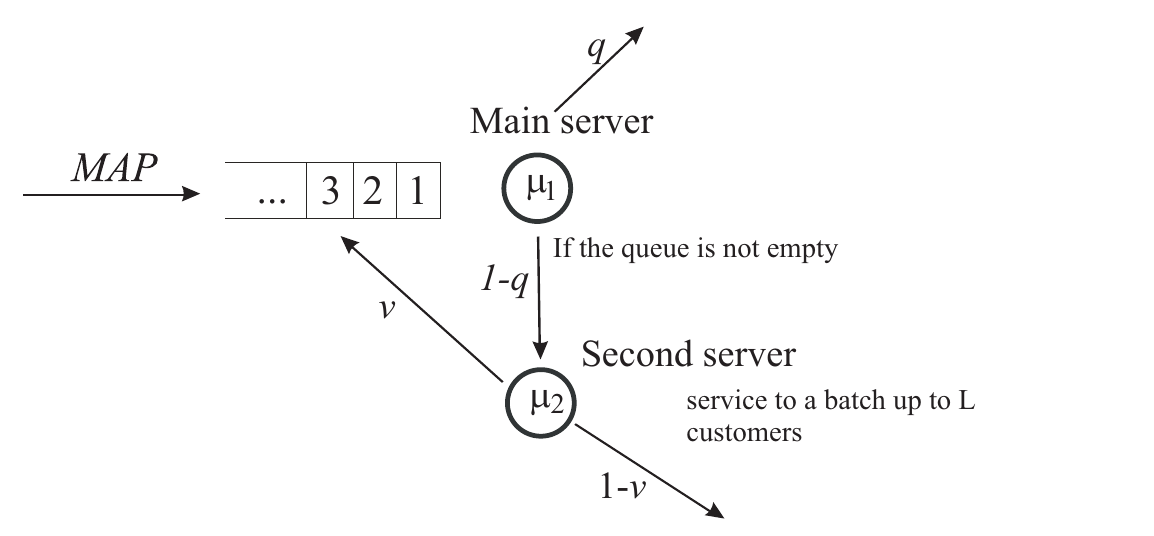
\includegraphics[width=\textwidth]{hVQg024.png}
        \caption{Immagine da [1]}
        \label{fig:diagramma_di_stato}
    \end{figure}
\end{frame}


\section{Studio del modello di coda in stato stazionario}


\begin{frame}
    \frametitle{Due approcci possibili}
    \begin{block}{QBD}
        Primo processo che analizzeremo in  questa sezione: un caso particolare delle catena di markov a tempo continuo (CTMC)
    \end{block}
    \begin{block}{GI/M/1}
        Una GI/M/1-type Markov chain assume che il tempo tra gli arrivi e il tempo di servizio dei clienti seguano una distribuzione generica, mentre è presente un solo server.
    \end{block}
\end{frame}


\subsection{QBD}


% \begin{frame}
%     \frametitle{Catena di Markov a tempo continuo (CTMC)}
%     \begin{block}{Definizione}
%         Il processo stocastico $\big\{X(t) : t \in \mathbb{R}^+\big\}$ in uno spazio di stati al più numberabile $E$ è un processo di Markov omogeneo se
%         $$ P[X(t+s) = j ~ | ~ X(u) : 0 \leq u \leq t] =  P[X(t+s) = j ~ | X(t)]$$
%         e se
%         $$  P[X(t+s) = j ~ | ~ X(t) = i] =  P[X(s) = j ~ | ~ X(0) = i]$$
%         per tutti gli stati $i, j \in E$, per tutti i tempi $t \geq 0$ e per tutti gli intervalli di tempo $s \geq 0$.
%     \end{block}
% \end{frame}


\begin{frame}
    \frametitle{Introduzione al QBD}
    \begin{block}{}
        Un \emph{quasi-death-birth process} (QBD) è un caso particolare di una catena di Markov a tempo continuo (CTMC). Ci sono due tipi di eventi che possono verificarsi: eventi di morte e eventi di nascita.
    \end{block}

    % \begin{itemize}
    %     \item Un evento di morte avviene quando un cliente lascia il sistema (i.e finisce di essere servito e se ne va)
    %     \item Un evento di nascita avviene quando un nuovo cliente entra nel sistema
    % \end{itemize}
\end{frame}


\begin{frame}
    \frametitle{Introduzione al QBD}
    \begin{block}{}
        Imponendo le restrizioni di entrambi i tipi di code $M/G/1$ che delle $G/M/1$, si vietano transizioni di più di livello alla volta, ottenendo così un processo QBD.
    \end{block}
    La matrice di transizione di tale processo è definita come segue:
    \begin{equation*}
        P=
        \begin{pmatrix}
            B_0 & B_1 & & & 0 \\
            A_{-1} & A_0 & A_1 & & \\
            & A_{-1} & A_0 & A_1 & \\
            & & A_{-1} & A_0 & \ddots \\
            0 & & & \ddots & \ddots
        \end{pmatrix}
        ,\quad A_{-1}, A_0, A_1, \in \mathbb{R}^{m \times m}, \quad B_0, B_1 \in \mathbb{R}^{m \times m}
    \end{equation*}
\end{frame}


\begin{frame}
    \frametitle{Generatore infinitesimale del processo QBD}
    \begin{block}{}
        Il generatore infinitesimale di un processo QBD è una matrice tridiagonale a blocchi infinita $Q$ che descrive la probabilità di transizione del sistema da uno stato $i$ ad uno stato $j$, in un dato istante di tempo $t$, attraverso un evento infinitesimo
    \end{block}
\end{frame}


% \begin{frame}
%     \frametitle{Introduzione al QBD}
%     \begin{block}{Generalizzazione del QBD}
%         Si potrebbe pensare al QBD come un semplice lista lineare in evoluzione: ogni livello è un nodo nella lista ed il processo è autorizzato a muoversi da un nodo ad uno dei suoi due vicini.
%     \end{block}
% \end{frame}


% \begin{frame}
%     \frametitle{Generatore infinitesimale del processo QBD}
%     \begin{block}{Proprietà degli elementi non diagonali}
%         Per tutte le $i \neq j$, $Q_{i,j}$ è il rate istantaneo di transizione dallo stato $i$ allo stato $j$. $Q_{i,j}$ è non negativo e strettamente positivo se è possibile spostarsi da $i$ a $j$ in un solo salto.
%     \end{block}
%     \begin{block}{Proprietà degli elementi diagonali}
%         Gli elementi diagonali sono tali che
%         $$Q_{i,i} = - \sum_{j \in E, j \neq i} Q_{i,j}$$
%         Se $Q_{i,i} = 0$, allora $Q_{i,j} = 0$ per tutti $j$, ciò significa che $i$ è uno stato assorbente.
%     \end{block}
% \end{frame}


\begin{frame}
    \frametitle{Generatore infinitesimale del processo QBD}
    Al tempo $t\geq 0$, indichiamo:
    \begin{itemize}
        \item $i_t\geq 0$ il numero di clienti nel sistema
        \item $n_t\in\{0,\ldots,\min(i_t,L)\}$ il numero di clienti in servizio al server secondario
        \item $\xi_t=1,\ldots,m$ lo stato del processo sottostante del \emph{MAP} che descrive gli arrivi dei clienti
    \end{itemize}
    \begin{block}{}
        Allora, il processo stocastico $\{\zeta_t=(i_t,n_t,\xi_t),,t\geq 0\}$ che descrive il comportamento del modello in esame è un CTMC regolare e irriducibile.
    \end{block}
\end{frame}


\begin{frame}
    \frametitle{Generatore infinitesimale del processo QBD}
    \begin{block}{}
        Enumerando gli stati della CTMC, $\{\zeta_t,t\geq 0\}$, in ordine lessicografico e indicando con $i$ il livello, per $i\geq 0$, definiamo l'insieme di stati come
        $$\{(i,n,k):0\leq n\leq \min(i,L),1\leq k\leq m\}$$
    \end{block}
\end{frame}


\begin{frame}
    \frametitle{Generatore infinitesimale del processo QBD}
    \begin{theorem}
        Il generatore infinitesimale $Q$ del processo stocastico CTMC $\{\zeta_t,,t\geq 0\}$ ha una struttura a blocchi tridiagonale come segue:
        \small{\begin{equation*}
            Q =
            \begin{pmatrix}
                Q_{0,0} & Q_{0,1} & 0 & 0 & \dots & 0 & 0& 0 & 0 & \dots \\
                Q_{1,0} & Q_{1,1} & Q_{1,2} & 0 & \dots & 0 & 0 & 0 & 0 & \dots \\
                0 & Q_{2,1} & Q_{2,2} & Q_{2,3} & \dots & 0 & 0 & 0 & 0 & \dots \\
                \vdots & \vdots & \vdots & \vdots & \ddots & \vdots & \vdots & \vdots & \vdots & \ddots \\
                0 & 0 & 0 & 0 & \dots & Q_{L,L-1} & Q_{L,L} & Q^+& 0 & \ddots \\
                0 & 0 & 0 & 0 & \dots & 0 & Q^- & Q^0 & Q^+ & \dots \\
                0 & 0 & 0 & 0 & \dots & 0 & 0 & Q^- & Q^0 & Q^+ \\
                \vdots & \vdots & \vdots & \vdots & \ddots & \vdots & \vdots & \vdots & \vdots & \ddots
            \end{pmatrix}
        \end{equation*}}
    \end{theorem}
\end{frame}


\begin{frame}
    \frametitle{Generatore infinitesimale del processo QBD}
    Dove i blocchi $Q_{i,i}$ sono definiti come segue:
    \begin{block}{}
        $$Q_{0,0} = D_0$$
    \end{block}
    \begin{block}{}
        $$ Q_{i,i} = I_{i+1} \otimes \nu \mu_2 E_i^{-} \otimes I_m - (\mu_1 \widehat{I}_i + \mu_2 (I_{i+1} - \overline{I_i})) \otimes I_m \qquad 1 \leq i \leq L$$
    \end{block}
\end{frame}

\begin{frame}
    \frametitle{Generatore infinitesimale del processo QBD}
    \begin{block}{}
        $$ Q_{i,i} = I_{i+1} \otimes \nu \mu_2 E_i^{-} \otimes I_m - (\mu_1 \widehat{I}_i + \mu_2 (I_{i+1} - \overline{I_i})) \otimes I_m \qquad 1 \leq i \leq L$$
    \end{block}
    Dove:
    \begin{itemize}
        \item [$\otimes$] indica il prodotto di Kronecker per matrici
        \item [$E_l^-$] è una matrice quadrata di dimensioni $l+1$ con $(E_l^-)_{k,k-1} = 1$ per $1 \leq k \leq l$ e tutte le altre componenti nulle.
        \item [$\widehat{I_l}$] è una matrice quadrata di dimensioni $l+1$ con $(\widehat{I_l})_{k,k} = 1$ per $0 \leq k \leq l-1$ e tutte le altre componenti nulle.
        \item [$\overline{I_l}$] è una matrice quadrata di dimensioni $l+1$ con $(\overline{I_l})_{0,0} = 1$ e tutte le altre componenti nulle.
    \end{itemize}
\end{frame}


\begin{frame}
    \frametitle{Generatore infinitesimale del processo QBD}
    Mentre abbiamo
    \begin{block}{}
        $$ Q_{i,i+1} = E_i^+ \otimes D_1 \qquad 0 \leq i \leq L-1 $$
    \end{block}
    \begin{block}{}
        $$ Q_{1,0} = (1-\nu) \mu_2 \widetilde{E}_1^- \otimes I_m + \mu_1 I_1^- \otimes I_m \qquad 1 \leq i \leq L $$
    \end{block}
    \begin{block}{}
        $$ Q_{i,i-1} = (1-\nu) \mu_2 \widetilde{E}_i^- \otimes I_m + q \mu_1 I_i^- \otimes I_m + (1-q) \mu_1 I_i^+ \otimes I_m \qquad 1 \leq i \leq L $$
    \end{block}
\end{frame}


\begin{frame}
    \frametitle{Generatore infinitesimale del processo QBD}
    Dove
    \begin{itemize}
        \item [$E_l^+$] è una matrice di dimensioni $(l+1) \times (l+2)$ con $(E_l^+)_{k,k} = 0$ per $0 \leq k \leq l$ e tutte le altre componenti nulle.
        \item [$\widetilde{E}_l^-$] è una matrice di dimensioni $(l+1) \times l$ con $(\widetilde{E}_l^-)_{k,k-1} = 1$ per $1 \leq k \leq l$ e tutte le altre componenti nulle.
        \item [$I_l^-$] è una matrice di dimensioni $(l+1) \times l$ con $(I_l^-)_{k,k} = 1$ per $0 \leq k \leq l-1$ e tutte le altre componenti nulle.
        \item [$I_l^+$] è una matrice di dimensioni $(l+1) \times l$ con  $(I_l^+)_{0,l-1} = 1, (I_l^+)_{k,k} = 1$ per $1 \leq k \leq l-1$ e tutte le altre componenti nulle.
    \end{itemize}
\end{frame}

% \begin{frame}
%     \frametitle{Descrizione del processo QBD che governa il sistema e il suo generatore}
%     Dove i blocchi $Q_{i,i}$ sono definiti come segue:
%     \begin{figure}[h]
%         \centering
%         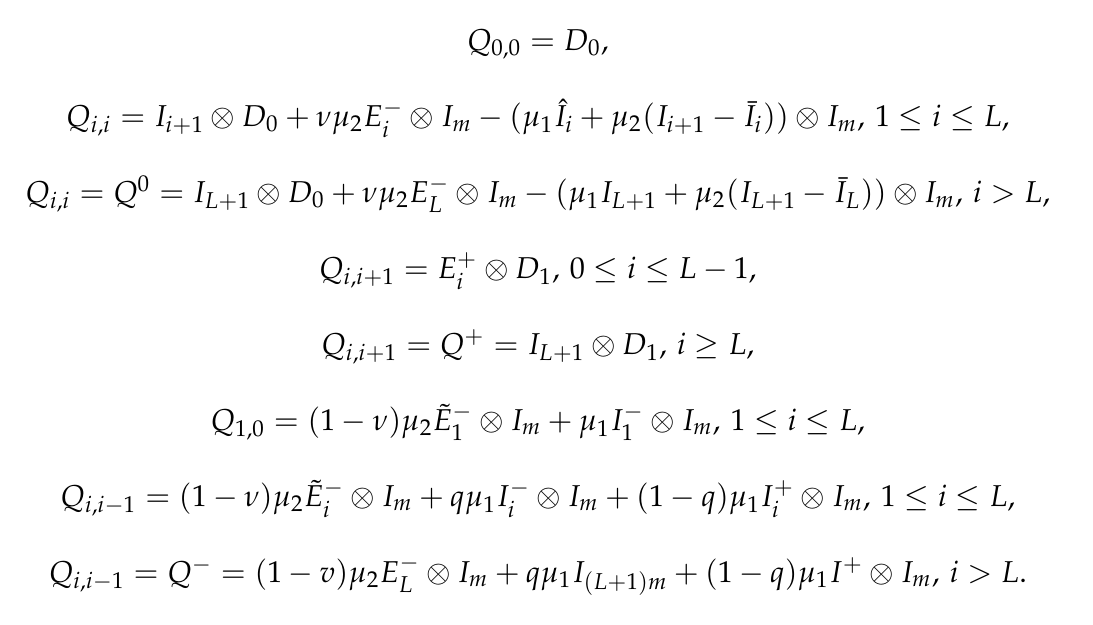
\includegraphics[width=0.9\textwidth]{T9RIVqa.png}
%     \end{figure}
% \end{frame}

\subsubsection{Condizione di ergodicità del processo QBD}

% \begin{frame}
%     \frametitle{Introduzione alla proprietà di ergodicità}
%     \begin{block}{Definizione}
%         Una catena di Markov si dice \emph{ergodica} se il limite
%         $$ \pi(j) = \lim_{n\to \infty} \mathbb{P}_i \{X_n = j\} $$
%         esiste per ogni stato $j$ e non dipende dallo stato iniziale $i$. Questo può anche essere scritto come
%         $$ \pi(j) = \lim_{n \to \infty} (P^n)_{i,j} $$
%     \end{block}
% \end{frame}

\begin{frame}
    \frametitle{Condizione di ergodicità del processo QBD}
    Il seguente risultato stabilisce la condizione di ergodicità del processo QBD che governa il sistema in esame.
    \begin{theorem}
        Il processo stocastico CTMC $\{\zeta_t,,t\geq 0\}$ è ergodico se e solo se vale la seguente disuguaglianza:
        \begin{equation*}\label{eq:ergodicity}
            \lambda < \mu_1 + \mu_2(1 - \nu) \frac{L(1-q)\mu_1}{L(1-q)\mu_1 + \mu_2}
        \end{equation*}
    \end{theorem}
\end{frame}

\begin{frame}
    \frametitle{Dimostrazione del teorema}
    \begin{block}{Dimostrazione}
        \small{Il criterio per l'ergodicità del QBD con il generatore di forma data come nel teorema precedente soddisfa l'ineguaglianza:
        \begin{equation*}
            y Q^- e > y Q^+e
        \end{equation*}}
        dove il vettore $y$ è l'unica soluzione del sistema
        \small{\begin{equation*}
            y(Q^- + Q^0 + Q^+) = \textbf{0}, \qquad ye = 1
        \end{equation*}}
        con
        \small{\begin{equation*}
            Q^+ = I_{L+1} \otimes D_1, \qquad i \geq L
        \end{equation*}
        \begin{equation*}
            Q^- = (1-\nu) \mu_2 E_L^- \otimes I_m + q \mu_1 I_{(L+1)m} + (1-q)\mu_1I^+ \otimes I_m \qquad i > L
        \end{equation*}
        \begin{equation*}
            Q^0 = I_{L+1} \otimes D_0 + \nu \mu_2 E_L^{-} \otimes I_m - (\mu_1 I_{L+1} + \mu_2(I_{L+1} - \overline{I}_L)) \otimes I_m \qquad i > L
        \end{equation*}}

    \end{block}
\end{frame}


\begin{frame}
    \frametitle{}
    \begin{block}{Dimostrazione}
        Si può inoltre verificare che
        \begin{equation*}\label{eq:bigotimes}
            Q^- + Q^0 + Q^+ = I_{L+1} \otimes (D_0 + D_1) + S \otimes I_{m}
        \end{equation*}
        dove
        \begin{equation*}
            S =
            \begin{pmatrix}
                -\mu_1 (1-q) & 0 & 0 & \dots & 0 \mu_1(1-q) \\
                \mu_2 & -\mu_2 & 0 & \dots & 0 & 0 \\
                0 & \mu_2 & -\mu_2 & \dots & 0 & 0 \\
                \vdots & \vdots & \vdots & \ddots & \vdots & \vdots \\
                0 & 0 & 0 & \dots & \mu_2 & -\mu_2 \\
            \end{pmatrix}
        \end{equation*}
    \end{block}
\end{frame}

\begin{frame}
    \frametitle{}
    \begin{block}{Dimostrazione}
            dove usando le regole del mixed product per il prodotto di Kronecker, e ricordando che
            $$ \delta(D_0 + D_1) = 0, \qquad \delta e = 1 $$
            si verifica che
            $$ y = x \otimes \delta $$
            dove $x$ è soluzione del sistema
            $$xS = 0, \qquad xe = 1 $$
    \end{block}
\end{frame}


\begin{frame}
    \frametitle{}
    \begin{block}{Dimostrazione}
        per sostituzione diretta, verifichiamo che le componenti del vettore $x = (x_0, x_1, ... , x_L)$, corrispondenti alle uniche soluzioni del sistema visto prima, sono date da
        \begin{equation*}
            x_0 = \frac{\mu_2}{L(1-q)\mu_1 + \mu_2}, \qquad x_i = \frac{\mu_1(1-q)}{L(1-q)\mu_1 + \mu_2}, \qquad i = 1, ..., L
        \end{equation*}
        La tesi segue delle equazioni viste in precedenza assieme alla definizione di $\lambda$.
        \qed
    \end{block}
\end{frame}


\begin{frame}
    \frametitle{Osservazioni sulla dimostrazione}
    \begin{block}{Osservazione 1}
        \begin{itemize}
            \item La condizione di ergodicità richiede che il tasso di arrivo dei clienti per unità di tempo debba essere inferiore al tasso di servizio che i clienti ricevono per unità di tempo quando il sistema è sovraccarico.
            \item Il tasso di servizio medio totale nel modello di coda è dato dalla somma del tasso di servizio fornito dal server principale e del tasso di servizio fornito dal server secondario.
        \end{itemize}
        Possiamo esprimere il tasso di servizio medio totale come segue:
        $$\mu = \mu_1 + \mu_2(1 - \nu) \frac{L(1-q)\mu_1}{L(1-q)\mu_1 + \mu_2}$$
    \end{block}
\end{frame}

\begin{frame}
    \frametitle{Osservazioni sulla dimostrazione}
    \begin{block}{Osservazione 2}
        Calcoliamo la probabilità $x_0$ che il secondo server non sia presente nel sistema in un qualsiasi momento in cui il sistema è sovraccarico.

        \begin{itemize}
            \item  Quando il sistema attiva un server secondario la durata media del server secondario continuamente presente nel sistema è data da $\frac{L}{\mu_2}$. Pertanto, abbiamo:
            \begin{equation*}
                x_0  = \frac{\frac{1}{\mu_1(1-q)}}{\frac{1}{\mu_1(1-q)} + \frac{L}{\mu_2}} = \frac{\mu_2}{L(1-q)\mu_1 + \mu_2}
            \end{equation*}
        \end{itemize}
    \end{block}
\end{frame}

\subsubsection{Calcolo della distribuzione stazionaria del processo QBD}

\begin{frame}
    \frametitle{Probabilità stazionarie}
    \begin{block}{}
         \begin{center}
            La distribuzione stazionaria di una CTMC irriducibile ricorrente è la distribuzione di probabilità a cui il processo converge per valori grandi di $t$.
         \end{center}
        % In altre parole, la distribuzione stazionaria è la distribuzione di probabilità di trovare il sistema in uno stato particolare quando il tempo tende all'infinito.
    \end{block}
    In particolare, per un processo QBD con n stati, la distribuzione stazionaria è un vettore di probabilità
    $$\pi = (\pi_1, \pi_2, ..., \pi_n)$$
    dove ogni $\pi_i$ rappresenta la probabilità di trovare il sistema nello stato $i$.
\end{frame}


\begin{frame}
    \frametitle{Probabilità stazionarie}
    Sotto l'assunzione che la condizione di ergodicità sia valida, esistono le seguenti probabilità stazionarie degli stati del CTMC $\{\zeta_t, t \geq 0\}$:
    $$\pi(i,n,\xi) = \lim_{t \to \infty} P\{i_t = i, n_t = n, \xi_t = \xi\}, ~ i \geq 0$$
    % $$n \in \{0, 1, \dots , \min\{i,L\}\}, \quad \zeta \in \{0, \dots, n\}$$
    Consideriamo i vettori riga delle probabilità di stato stazionario $\pi_i$ come segue
    \begin{block}{}
        $$\pi_i = (\pi(i,0), ..., \pi(i, \min \{i,L\})), \quad i \geq 0$$
    \end{block}
    dove
    $$\pi(i,n) = (\pi(i,n,1), ..., \pi(i,n,m))$$
\end{frame}


\begin{frame}
    \frametitle{Probabilità stazionarie}
    Sappiamo che i vettori di probabilità stazionari $\pi_i, i \geq 0$, soddisfano il sistema di equazioni algebriche lineari (equazioni di equilibrio):
    \begin{block}{}
        $$(\pi_0, \pi_1, \pi_, \dots)Q = 0 \qquad (\pi_0, \pi_1, \pi_, \dots)\textbf{e} = 1$$
    \end{block}
    dove $Q$ è la matrice di transizione del CTMC $\{\zeta_t, t \geq 0\}$ ed $\textbf{e}$ è il vettore colonna di tutti gli elementi $1$
\end{frame}

% La soluzione del problema di calcolo della distribuzione stazionaria di una QBD indipendente dal livello è ben nota; si veda [37]. Per i livelli in cui le transizioni della QBD non dipendono dal livello, i vettori di probabilità stazionaria sono trovati in forma matriciale geometrica. I vettori di probabilità stazionaria dei livelli di confine, in cui le transizioni della QBD dipendono dal livello, sono quindi direttamente trovati come soluzione del sistema di equazioni algebriche lineari. Tuttavia, se il numero di livelli di confine è grande (cosa che accade nel nostro modello se $L$ è grande), questo sistema ha una grande dimensione

\begin{frame}
    \frametitle{Algoritmo per risolvere il sistema di equazioni di equilibrio}
    \begin{block}{Goal}
            Vediamo un algoritmo che sfrutta la struttura tridiagonale a blocchi del generatore, ma dipendente dal livello, per risolvere più efficientemente il sistema di equazioni lineari algebriche quando il numero di livelli di confine è elevato.
    \end{block}
\end{frame}


\begin{frame}
    \frametitle{Algoritmo per risolvere il sistema di equazioni di equilibrio}
    \begin{theorem}
        I vettori $\pi_i, i \geq 0$, sono trovati come soluzione del sistema di equazioni algebriche lineari:
        \small{\begin{equation*}
            \pi_i = \alpha_i \big( \sum_{l=0}^\infty \alpha_l e \big)^{-1}, \qquad i \geq 0
        \end{equation*}}
        dove il vettore $\alpha_0$ è calcolato come l'unica soluzione del sistema di equazioni
        \small{\begin{equation*}
            \alpha_0(Q_{0,0} + Q_{0,1}G_0) = 0, \qquad \alpha_0e = 1
        \end{equation*}}
        ed i vettori $\alpha_i, i \geq 1$, sono definiti come
        \small{\begin{equation*}
            \alpha_i = \alpha_0 \prod_{l=1}^i R_l, \qquad i \geq 1
        \end{equation*}}
    \end{theorem}
\end{frame}


\begin{frame}
    \frametitle{Algoritmo per risolvere il sistema di equazioni di equilibrio}
    \begin{theorem}
        Altrimenti tramite la formula ricorsiva
        \begin{equation*}\label{eq:rec-alpha}
            \alpha_i = \alpha_{i-1} R_i, \qquad i \geq 1
        \end{equation*}
        dove
        \begin{equation*}
            R =
            \begin{cases}
                -Q_{i-1,i}(Q_{i,i} + Q_{i,i+1}G_i)^{-1}Q & 1 \leq i \leq L-1 \\
                -Q_{L-1,L}(Q_{L,L} + Q^+G)^{-1} & i = L \\
                -Q^+(Q^0 + Q^+G)^{-1} = R & i>L
            \end{cases}
        \end{equation*}
    \end{theorem}
\end{frame}


\begin{frame}
    \frametitle{Algoritmo per risolvere il sistema di equazioni di equilibrio}
    \begin{theorem}
        Le matrici stocastiche $G_i$ sono calcolate utilizzando la seguente formula ricorsiva all'indietro:
            $$G_L = G$$
            $$G_{L-1} = -(Q_{L,L} + Q^+G_L)^{-1}Q_{L,L-1}$$
            $$G_i = -(Q_{i+1,i+1} + Q_{i+1,i+2}G_{i+1})^{-1}Q_{i+1,i}, \qquad i = L-2, L-3, \dots, 0$$
        dove la matrice $G$ è la minima soluzione non negativa dell'equazione quadratica matriciale
        \begin{equation*}
            Q^+G^2 + Q^0G + Q^- = 0
        \end{equation*}
    \end{theorem}
\end{frame}


\begin{frame}
    \frametitle{Algoritmo per risolvere il sistema di equazioni di equilibrio}
    \begin{itemize}
        \item L'algoritmo proposto è una modifica dell'algoritmo per il calcolo della distribuzione stazionaria di una CTMC asintotica quasi-Toeplitz.
        % \item Utilizzando la ricorsione di vettori anziché quella di matrici si ha una significativa riduzione della complessità in tempo e spazio.
        \item Le inverse delle matrici utilizzate nell'algoritmo sono sub-generatori irriducibili e semi-stabili, il che rende stabile l'implementazione numerica dell'algoritmo.
    \end{itemize}
\end{frame}


% \subsection{GI/M/1}


% \begin{frame}{Introduzione alle code di tipo GI/M/1}
%     \begin{block}{}
%         Una coda di tipo GI/M/1 è un processo stocastico che modella il comportamento di un sistema di code con un singolo server
%     \end{block}
%     \begin{itemize}
%         \item [GI] \emph{General inter-arrival time distribution} distribuzione del tempo tra gli arrivi dei clienti alla coda.
%         \item [M] \emph{Markovian service time distribution}: si riferisce alla distribuzione dei tempi di servizio per ciascun cliente, che viene assunta essere un processo di Markov.
%         \item [1] \emph{One server}: un solo server nel sistema, e che solo un cliente alla volta può essere servito.
%     \end{itemize}
% \end{frame}


% \begin{frame}
%     \frametitle{Code di tipo GI/M/1}
%     \begin{block}{}
%             Definiamo come prima cosa lo spazio degli stati $\Omega$ del CTMC come:
%             $$\Omega = \{ (i,j,k) ~ : ~ i \geq 0, 0 \leq j \leq K, 1 \leq k \leq m \}$$
%     \end{block}
%     Definiamo il livello \textbf{i} come:
%     \begin{equation*}
%         \textbf{i} = \{(i, j, k) : 0 \leq j \leq L, 1 \leq k \leq m\} = \{(\textbf{i}, 0), \dots, (\textbf{i}, L)\}, \quad i \geq 0
%     \end{equation*}
% \end{frame}


% \begin{frame}
%     \frametitle{Code di tipo GI/M/1}
%     \begin{block}{Osservazione}
%         \begin{itemize}
%             \item il livello $(\textbf{i},\textbf{j})$ indica che il server principale è occupato, ci sono $i-1$ clienti in attesa nella coda principale; il server secondario è occupato e il processo di arrivo si trova in varie fasi
%             \item  Il livello $(\textbf{0},\textbf{0})$ corrisponde al sistema inattivo con il processo \emph{MAP} in una delle $m$ fasi.
%         \end{itemize}
%     \end{block}
% \end{frame}


% \begin{frame}
%     \frametitle{Il generatore del CTMC}
%     Il generatore $\widetilde{Q}$ della CTMC che governa il sistema in studio è:
%     \begin{figure}
%         \centering
%         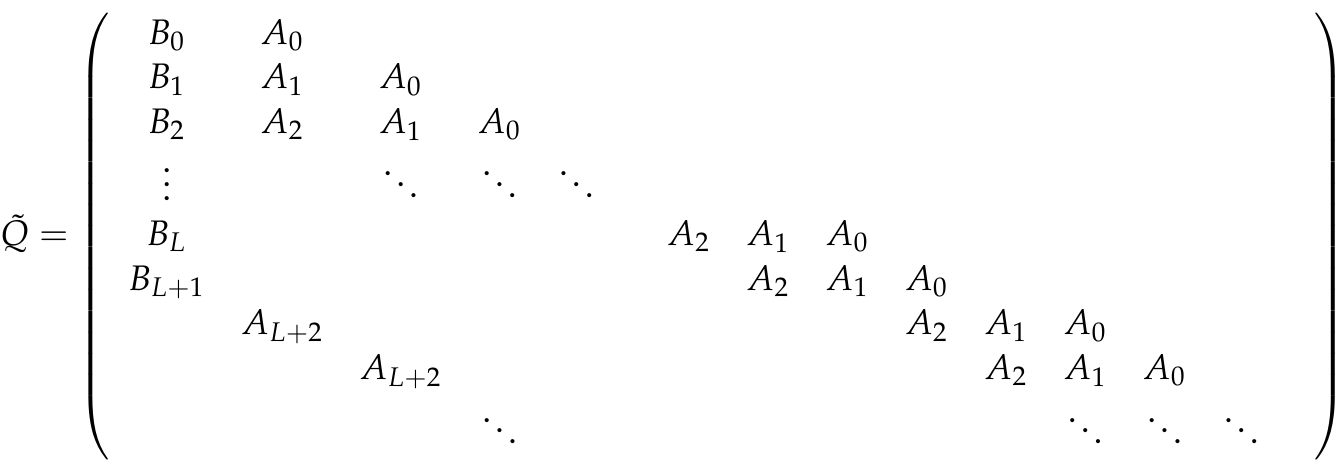
\includegraphics[width=\textwidth]{Isy9B7s.png}
%     \end{figure}
% \end{frame}


% \begin{frame}
%     \frametitle{Il generatore del CTMC}
%     Dove abbiamo:
%     \begin{equation*}
%         B_0 =
%         \begin{pmatrix}
%             D_0 & & & & \\
%             \widetilde{\nu}\mu_2 I & D_0 - \mu_2 I & & & \\
%             & \widetilde{\nu}\mu_2 I & D_0 - \mu_2 I & & \\
%             & & \ddots & \ddots & \\
%             & & & \widetilde{\nu}\mu_2 I & D_0 - \mu_2 I
%         \end{pmatrix}
%     \end{equation*}
% \end{frame}


% \begin{frame}
%     \frametitle{Il generatore del CTMC}
%     Dove abbiamo:
%     \begin{equation*}
%         \begin{split}
%             A_0 &=
%             \begin{pmatrix}
%                 D_1 & & & & \\
%                 \nu\mu_2 I & D_1 & & & \\
%                 & \nu \mu_2 I & D_1 & & \\
%                 & & \ddots & \ddots & \\
%                 & & & \nu \mu_2 I & D_1
%             \end{pmatrix} \\
%             A_1 &= B_0 -\mu_1 I \\
%             A_2 & = \mu_1 \Delta(q,1, \dots, 1) \\
%             B_1 &= \mu_1 I \\
%             B_r &= \rho \mu_1 (e_r^T \otimes e(L+1)) \qquad 2 \leq r \leq L+1 \\
%             A_{L+2} &= B_{L+1}
%         \end{split}
%     \end{equation*}
% \end{frame}


% \begin{frame}
%     \frametitle{Proprietà delle queue di tipo GI/M/1}
%     Utilizzando i risultati per le code di tipo G1/M/1 in tempo continuo, si verificano le seguenti proprietà:
%     \begin{block}{Proprietà 1}
%         Sia
%         $$\widetilde{y} = (\widetilde{y_0}, \dots, \widetilde{y_{L}})$$
%         il vettore invariante di $\displaystyle A = \sum_{i=0}^{L+2} A_i$. Allora:
%             $$ \widetilde{y_0} = \delta(\mu_2I - D_0 - D_1)[\mu_2U + L\rho\mu_1 I - D_0 - D_1]^{-1} $$
%             $$ \widetilde{y_r} = \rho \mu_1 \pi_0(\mu_2I - D_0 - D_1)^{-1}, \qquad 1 \leq r \leq L $$
%     \end{block}
% \end{frame}


% \begin{frame}
%     \frametitle{Proprietà delle queue di tipo GI/M/1}
%     \begin{block}{Proprietà 2}
%         La condizione di stabilità
%         $$ \widetilde{y} A_0 e < \widetilde{y} \sum_{i=1}^{L+2}(i-1)A_i e $$
%         si riduce alla disuguaglianza vista prima:
%         $$ \lambda < \mu_1 + \mu_2(1 - \nu) \frac{L(1-q)\mu_1}{L(1-q)\mu_1 + \mu_2}  $$
%     \end{block}
% \end{frame}


% \begin{frame}
%     \frametitle{Proprietà delle queue di tipo GI/M/1}
%     \begin{block}{Proprietà 3}
%         Data $R$ la matrice di rate, soddisfa l'equazione matriciale non lineare data da:
%         $$ R^{L+2} A_{L+2} + R^2A_2 + RA_1 + A_0 = 0 $$
%     \end{block}
% \end{frame}


% \begin{frame}
%     \frametitle{Proprietà delle queue di tipo GI/M/1}
%     \begin{block}{Proprietà 4}
%         Indicando con $\widetilde{\pi}$ il vettore di probabilità stazionario del generatore $\widetilde{Q}$ come visto prima, otteniamo qui la soluzione matriciale geometrica classica:
%         $$ \widetilde{\pi}_i = \widetilde{\pi}_0R^i, \qquad i \geq 1 $$
%         dove $\widetilde{\pi}_0$ è ottenuto risolvendo il seguente sistema di equazioni lineari:
%         $$ \widetilde{\pi}_0\Bigg[ \sum_{i=0}^{L+1} R^iB_i \Bigg] = 0, \qquad \widetilde{\pi}_0e = 1 $$
%     \end{block}
% \end{frame}


\section{Risultati Numerici}
\begin{frame}
    \frametitle{Introduzione ai risultati numerici}
    Vedremo 3 esempi illustrativi utilizzando 5 processi di arrivo. In particolare i 5 \emph{MAP} considerati sono:
    \begin{block}{1. ERL}
        Erlang di ordine 5 con parametro 2.5 in ciascuno dei 5 stati. Prendiamo poi $\lambda = 0.5, \sigma = 0.899427$ e $\rho_c = 0$.
    \end{block}
    \begin{block}{2. EXP}
        Un esponenziale con una frequenza di 0.5. Prendiamo poi $\lambda = 0.5, \sigma = 2$ e $\rho_c = 0$.
    \end{block}
\end{frame}


\begin{frame}
    \frametitle{}
    \begin{block}{3. HEX}
        Distribuzione iper-esponenziale con una probabilità di mixing data da (0.5, 0.3, 0.15, 0.04, 0.01) con i corrispondenti tassi della distribuzione esponenziale pari a (1.09, 0.545, 0.2725, 0.13625, 0.068125). Qui abbiamo $\lambda = 0.5, \sigma = 3.3942$ e $\rho_c = 0$.
    \end{block}
\end{frame}


\begin{frame}
    \frametitle{}
    \begin{block}{4. NCR}
        \emph{MAP} negativamente correlato, con matrici di rappresentazione:
        \small{\begin{equation*}
            D_0 =
            \begin{pmatrix}
                -1.125 & 0.125 & 0 & 0 & 0 \\
                0 & -1.125 & 0.125 & 0 & 0 \\
                0 & 0 & -1.125 & 0.125 & 0 \\
                0 & 0 & 0 & -0.125 & 0 \\
                0 & 0 & 0 & 0 & -2.25
            \end{pmatrix}
        \end{equation*}
        \begin{equation*}
            D_1 =
            \begin{pmatrix}
                0 & 0 & 0 & 0 & 0 \\
                0 & 0 & 0 & 0 & 0 \\
                0 & 0 & 0 & 0 & 0 \\
                0.01125 & 0 & 0 & 0 & 1.11375 \\
                2.2275 & 0 & 0 & 0 & 0.0225
            \end{pmatrix}
        \end{equation*}}
        dove abbiamo $\lambda = 0.5, \sigma = 2.02454$ e $\rho_c =  -0.57855$
    \end{block}
\end{frame}


\begin{frame}
    \frametitle{}
    \begin{block}{5. PCR}
        \emph{MAP} positivamente correlato, con matrici di rappresentazione:
        \small{\begin{equation*}
            D_0 =
            \begin{pmatrix}
                -1.125 & 0.125 & 0 & 0 & 0 \\
                0 & -1.125 & 0.125 & 0 & 0 \\
                0 & 0 & -1.125 & 0.125 & 0 \\
                0 & 0 & 0 & -0.125 & 0 \\
                0 & 0 & 0 & 0 & -2.25
            \end{pmatrix}
        \end{equation*}
        \begin{equation*}
            D_1 =
            \begin{pmatrix}
                0 & 0 & 0 & 0 & 0 \\
                0 & 0 & 0 & 0 & 0 \\
                0 & 0 & 0 & 0 & 0 \\
                1.11375 & 0 & 0 & 0 & 0.01125 \\
                0.0225 & 0 & 0 & 0 & 2.2275
            \end{pmatrix}
        \end{equation*}}
        dove abbiamo $\lambda = 0.5, \sigma = 2.02454$ e $\rho_c =  0.57855$
    \end{block}
\end{frame}


\begin{frame}
    \frametitle{Introduzione ai risultati numerici}
    \begin{block}{Osservazioni}
        \begin{itemize}
            \item Le cinque \emph{MAP} sopra riportate sono qualitativamente diverse.
            \item Il processo di arrivo \textbf{PCR} è ideale per situazioni di arrivi altamente irregolari con periodi di alta e bassa attività.
        \end{itemize}
    \end{block}
\end{frame}


\begin{frame}
    \frametitle{Primo esempio illustrativo}
    \begin{block}{Obiettivo}
        Discutiamo l'impatto del parametro $L$ su alcune misure di performance del sistema per tutti e 5 i \emph{MAPs}
    \end{block}
    Fissiamo $\mu_1=1$, $\mu_2=0.5$, $q=0.5$, e $\nu=0.4$, e variamo $L$ da 1 a 30.
\end{frame}

\begin{frame}
    \frametitle{Primo esempio illustrativo}
    \begin{block}{$L_{\mathrm{sec}}$}
        Definiamo $L_{\mathrm{sec}}$ come il numero medio di clienti nel sistema con server secondari ad un momento arbitrario come:
        $$ L_{\mathrm{sec}} = \sum_{i=1}^{\infty} \sum_{n=1}^{\min\{i,L\}} n \pi (i,n) e $$
    \end{block}
    \begin{block}{$L_{\mathrm{system}}$}
        Definiamo $L_{\mathrm{system}}$ come il numero medio di clienti nell'intero sistema come:
        $$ L_{\mathrm{syste}} = \sum_{i=1}^{\infty} i \pi_i e $$
    \end{block}
\end{frame}

\begin{frame}
    \frametitle{Primo esempio illustrativo}
    \begin{figure}[h]
        \centering
        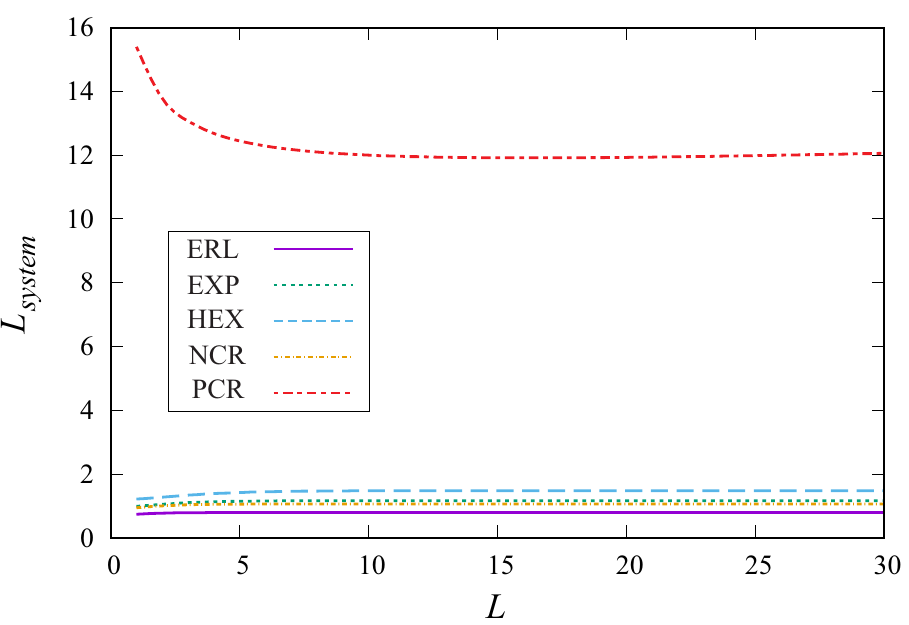
\includegraphics[width=0.75\textwidth]{gtHnIzQ.png}
        \caption{Impatto di $L$ sul numero medio di clienti nel sistema $L_{system}$ per diversi \emph{MAPs}}
        \label{fig:1}
    \end{figure}
\end{frame}


% \begin{frame}
%     \frametitle{Primo esempio illustrativo}
%         \begin{itemize}
%             \item Il \textbf{PCR} ha un alto numero medio di clienti nel sistema rispetto ad altri processi di arrivo.
%             \item $L$ aumenta il numero medio di clienti nel sistema per i primi quattro \emph{MAP}, ma per il \textbf{PCR} il trend non è crescente a causa della correlazione positiva.
%             \item Alti valori di $L$ aumentano la probabilità di avere più clienti nel sistema, soprattutto per i primi quattro \emph{MAP}.
%             \item Per gli arrivi \textbf{PCR}, $L$ diminuisce il numero medio di clienti nel sistema perché i server secondari aiutano a ripulire la coda.
%         \end{itemize}
% \end{frame}


\begin{frame}
    \frametitle{Primo esempio illustrativo}
    \begin{figure}[h]
        \centering
        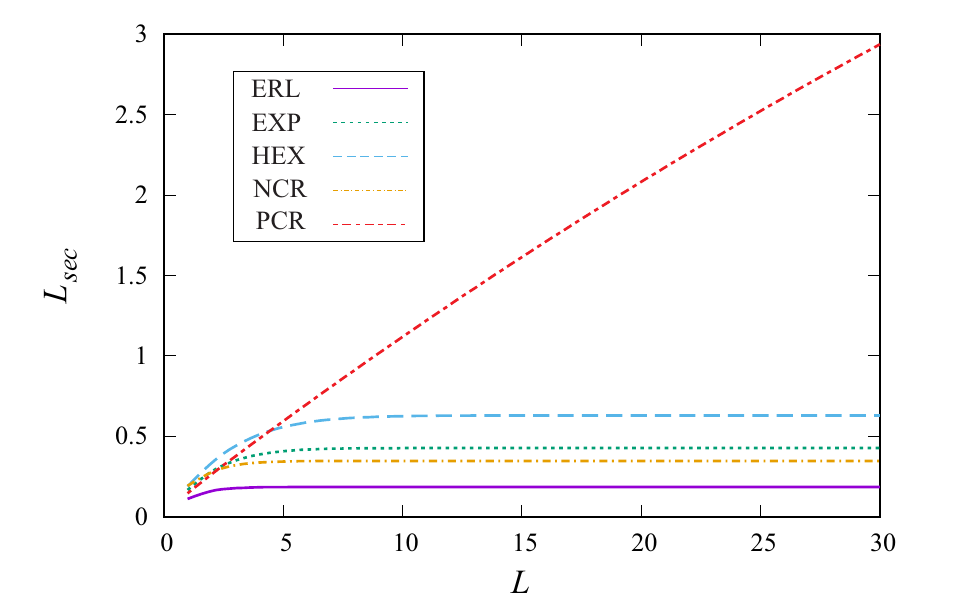
\includegraphics[width=0.8\textwidth]{Tcjl81t.png}
        \caption{Dipendenza del numero medio di clienti con il server secondario $L_{\mathrm{sec}}$ al variare di $L$ per diversi \emph{MAPs}}
        \label{fig:2}
    \end{figure}
\end{frame}


% \begin{frame}
%     \frametitle{Primo esempio illustrativo}
%         \begin{itemize}
%             \item $L_{\mathrm{sec}}$ aumenta all'aumentare di L, come previsto.
%             \item Il valore di $L_{\mathrm{sec}}$ è elevato per \textbf{PCR} e solo per valori piccoli di L è inferiore per \textbf{ERL-NCR}.
%             \item L'alta irregolarità degli arrivi nel processo \textbf{PCR} causa la "fame" del sistema, durante la quale solo il server primario è occupato offrendo servizi per la maggior parte dei clienti.
%         \end{itemize}
% \end{frame}


\begin{frame}
    \frametitle{Primo esempio illustrativo}
    \begin{block}{$P_{\mathrm{idle-system}}$}
        Definiamo la probabilità che il sistema sia in equilibrio ad un momento arbitrario come:
        $$  P_{\mathrm{idle-system}} = \pi_0 e $$
    \end{block}
\end{frame}


\begin{frame}
    \frametitle{Primo esempio illustrativo}
    \begin{figure}[h]
        \centering
        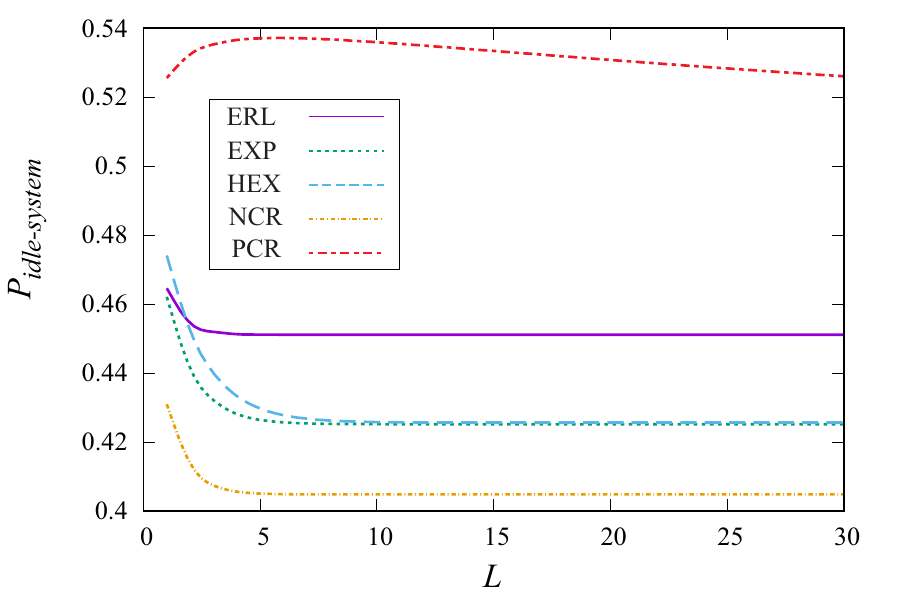
\includegraphics[width=0.8\textwidth]{pSUZiNk.png}
        \caption{Dipendenza della probabilità $P_{\mathrm{idle-system}}$ rispetto ad $L$ che il sistema sia in idle ad un momento arbitrario, per diversi \emph{MAPs}}
        \label{fig:3}
    \end{figure}
\end{frame}


% \begin{frame}
%     \frametitle{Primo esempio illustrativo}
%         \begin{itemize}
%             \item Esiste una grande differenza nella misura a seconda dei diversi \emph{MAPs} utilizzati.
%             \item Il valore ottimale di $L$ dipende dall'obiettivo: ad esempio, per il processo di arrivo \textbf{PCR}, il valore ottimale di $L$ è $16$ se si cerca di minimizzare $L_{\mathrm{system}}$, ma è 6 se si massimizza $P_{\mathrm{idle-system}}$.
%         \end{itemize}
% \end{frame}

\begin{frame}
    \frametitle{Primo esempio illustrativo}
    \begin{block}{$P_{\mathrm{idle-busy}}$}
        Definiamo la probabilità che il main server sia in idle quando il server secondario è occupato come:
        $$ P_{\mathrm{idle-busy}} = \sum_{n=1}^{L} \pi(n,n) e $$
    \end{block}
    \begin{block}{$P_{\mathrm{busy-idle}}$}
        Definiamo la probabilità che il main server sia occupato quando il server secondario è in idle come:
        $$ P_{\mathrm{busy-idle}} = \sum_{i=0}^{\infty} \pi(i,0) e $$
    \end{block}
\end{frame}

\begin{frame}
    \frametitle{Primo esempio illustrativo}
    \begin{figure}[h]
        \centering
        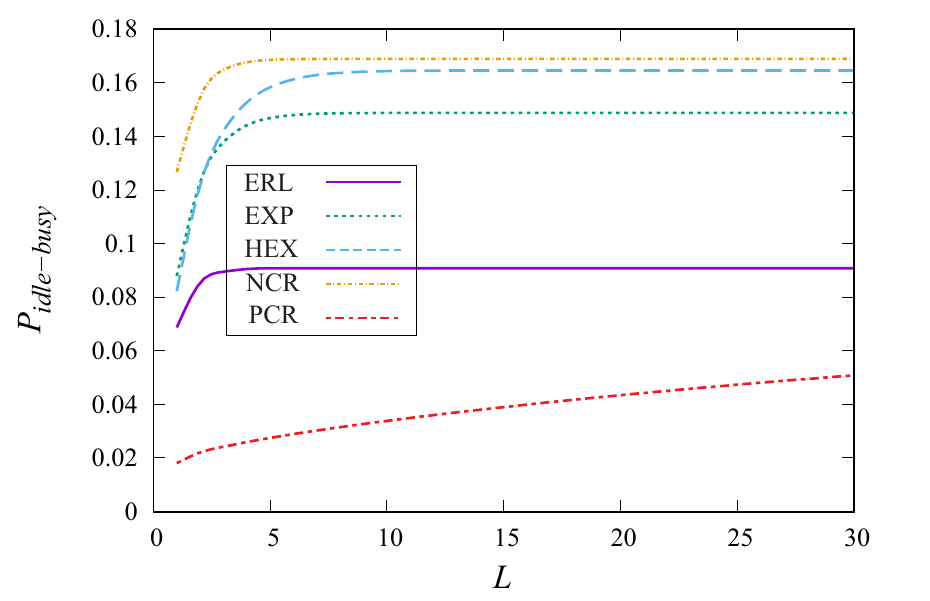
\includegraphics[width=0.75\textwidth]{VrxLKYI.png}
        \caption{Dipendenza della probabilità $P_{\mathrm{idle-busy}}$ rispetto ad $L$ che il main server sia in idle quando il server secondario è in occupato, per diversi \emph{MAPs}}
        \label{fig:4}
    \end{figure}
\end{frame}


\begin{frame}
    \frametitle{Primo esempio illustrativo}
    \begin{figure}
        \centering
        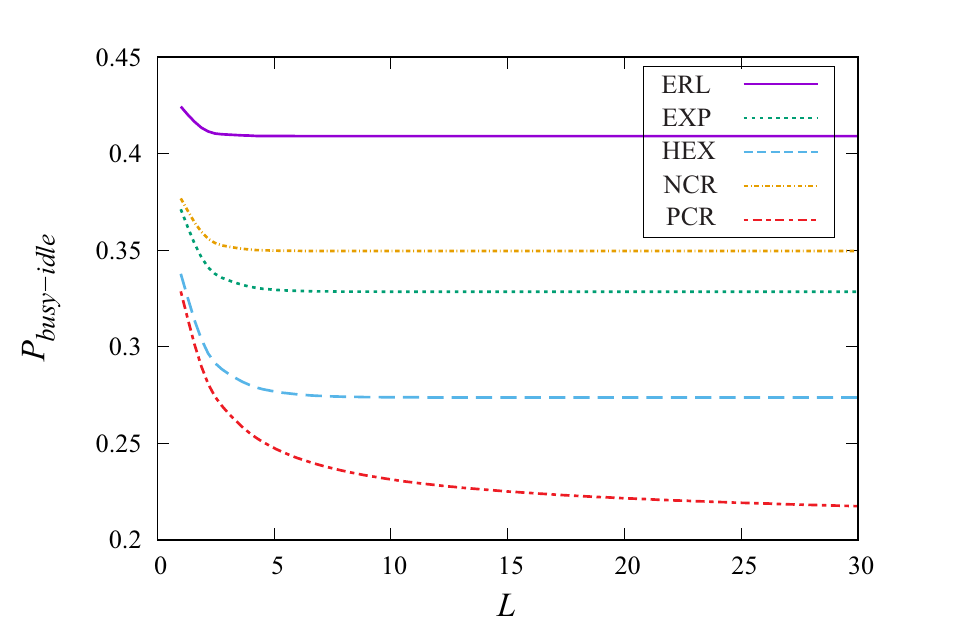
\includegraphics[width=0.75\textwidth]{EZp90oP.png}
        \caption{Dipendenza della probabilità $P_{\mathrm{busy-idle}}$ rispetto ad $L$ che il main server sia occupato quando il server secondario è in idle, per diversi \emph{MAPs}}
        \label{fig:5}
    \end{figure}
\end{frame}




\begin{frame}
    \frametitle{Secondo esempio illustrativo}
    \begin{block}{Obiettivi}
        L'obiettivo è valutare l'impatto dei parametri $q$ e $\nu$ sulla prestazione del sistema. Dove
        \begin{itemize}
            \item $q$ è la probabilità che un cliente servito si rifiuti di agire come server secondario
            \item $\nu$ è la probabilità che un cliente servito da un server secondario non sia soddisfatto e venga mandato indietro al server primario
        \end{itemize}

    \end{block}
    Fissiamo il valore di $L$ a $10$ e i tassi di servizio $\mu_1$ e $\mu_2$ a $1$ e $0.5$. Si variano i valori di $q$ e $\nu$ da $0$ a $1$ con passo $0.05$ e si analizza l'impatto sulle misure di prestazione del sistema.
\end{frame}


% \begin{frame}
%     \frametitle{Secondo esempio illustrativo}
%     \begin{block}{}
%         In questo esempio ci concentriamo sul processo di arrivo PCR, la cui scelta è basata sul comportamento di questo processo sulle misure evidenziato nel primo esempio illustrativo
%     \end{block}
% \end{frame}


\begin{frame}
    \frametitle{Secondo esempio illustrativo}
    \begin{figure}[h]
        \centering
        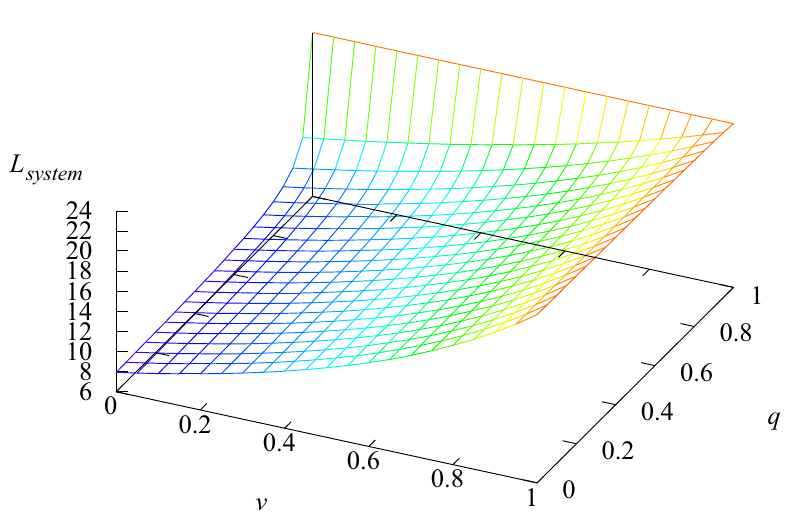
\includegraphics[width=0.8\textwidth]{qUQVrEZ.png}
        \caption{Dipendenza del numero medio di clienti nel sistema $L_{\mathrm{system}}$ rispetto a $q$ e $\nu$}
    \end{figure}
\end{frame}


% \begin{frame}
%     \frametitle{Secondo esempio illustrativo}
%     \begin{itemize}
%         \item L'analisi mostra che il valore di $L_\mathrm{system}$ è minimo a $7.9328$ quando $q$ e $\nu$ sono entrambi uguali a $0$.
%         \item Aumentando $q$ o $\nu$, il valore di $L_\mathrm{system}$ aumenta, con un aumento più veloce quando uno o entrambi si avvicinano a $1$.
%         \item Quando $q=1$, il sistema diventa un modello \emph{MAP}/M/1 classico e il valore di $L_\mathrm{system}$ diventa $22.30425$ per tutti i valori di $\nu$.
%         \item L'uso di un server secondario riduce il numero medio di clienti nel sistema di oltre il $40\%,$ e il punto di interruzione per il modello classico è $\nu^* \sim 0.985$.
%     \end{itemize}
% \end{frame}


\begin{frame}
    \frametitle{Secondo esempio illustrativo}
\begin{block}{Modifichiamo i parametri}
        \begin{itemize}
            \item Si aumenta $\lambda$ del 50\% a 0.75 per testare l'importo della riduzione del numero medio di clienti nel sistema.
            \item Mantenendo gli altri parametri costanti, si ottiene una riduzione superiore al 52,8\%.
            \item Ciò suggerisce che l'aggiunta di un server secondario beneficia notevolmente l'aumento del carico del sistema anche con un tasso di insoddisfazione del cliente del 50\%.
        \end{itemize}
\end{block}
\end{frame}


\begin{frame}
    \frametitle{Secondo esempio illustrativo}
    \begin{figure}[h]
        \centering
        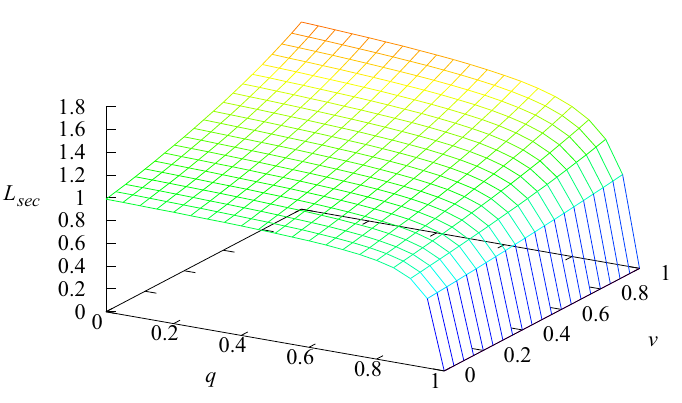
\includegraphics[width=0.8\textwidth]{0uFWo7C.png}
        \caption{ Dipendenza del numero medio di clienti nel sistema $L_{\mathrm{sec}}$ rispetto a $q$ e $\nu$ con $\lambda=0.75$}
    \end{figure}
\end{frame}


% \begin{frame}
%     \frametitle{Secondo esempio illustrativo}
%     \begin{itemize}
%         \item $L_\mathrm{sec}$ diminuisce significativamente quando $q$ si avvicina a $1$ e quando i clienti sono raramente reclutati per diventare server secondari.
%         \item $L_\mathrm{sec}$ ha il valore massimo quando $q$ è uguale a zero e $\nu$ è vicino a $1$, ma questo può creare ulteriore lavoro per il sistema e riflettersi negativamente sulla fornitura di servizi.
%     \end{itemize}
% \end{frame}


\begin{frame}
    \frametitle{Secondo esempio illustrativo}
    \begin{figure}[h!]
        \centering
        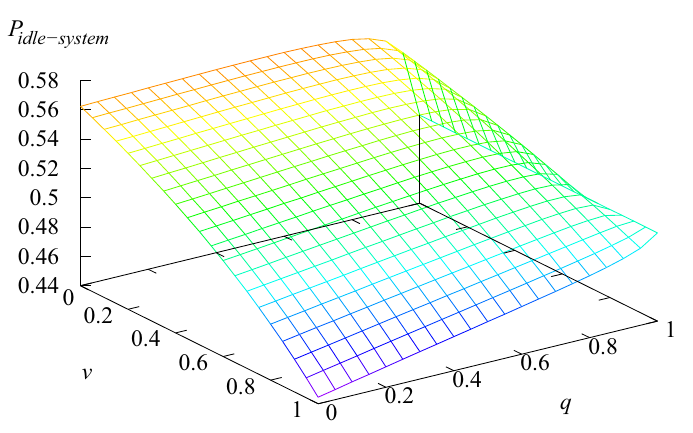
\includegraphics[width=0.8\textwidth]{3zlg6uj.png}
        \caption{Dipendenza della probabilità $P_\mathrm{idle-system}$ che il sistema sia in idle ad un momento arbitrario rispetto a $q$ e $\nu$.}
    \end{figure}
\end{frame}


% \begin{frame}
%     \frametitle{Secondo esempio illustrativo}
%     \begin{itemize}
%         \item $P_\mathrm{idle-system}$ ha il valore minimo di $0.4445$ quando $\nu=1$ e $q=0$, il che è intuitivo poiché servire nuovamente i clienti dopo aver passato attraverso un server secondario mette un carico sul sistema.
%         \item $P_\mathrm{idle-system}$ aumenta quando $q$ aumenta e/o $\nu$ diminuisce, con un valore massimo di $0.5652$ ottenuto quando $q=0.65$ e $\nu=0$.
%         \item Nel sistema \emph{MAP}/M/1 classico corrispondente, questa misura è $P_\mathrm{idle-system}=0.5$.
%     \end{itemize}
% \end{frame}


\begin{frame}
    \frametitle{Terzo esempio illustrativo}
    \begin{block}{Obiettivo}
        Analizzare l'impatto della variazione dei tassi di servizio $\mu_1$ e $\mu_2$ quando tutti gli altri parametri sono fissati.
    \end{block}
    \begin{itemize}
        \item I parametri fissati sono $L=10$, $q=0.5$, $\nu=0.4$, e $\lambda=0.5$.
        \item I tassi $\mu_1$ e $\mu_2$ vengono variati da $0.25$ a $2.0$ con incrementi di $0.05$, ma per soddisfare la condizione di ergodicità, il valore di $\mu_2$ viene limitato quando $\mu_1$ è piccolo.
        \item Solo per $\mu_1\geq0.4$, il valore di $\mu_2$ può essere variato da $0.25$, come originariamente indicato
    \end{itemize}
\end{frame}


\begin{frame}
    \frametitle{Terzo esempio illustrativo}
    \begin{figure}[h]
        \centering
        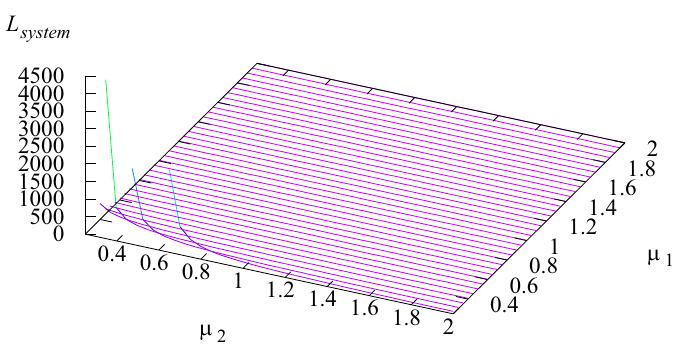
\includegraphics[width=0.8\textwidth]{9LBRzWR.png}
        \caption{Dipendenza del numero medio di clienti nel sistema $L_{\mathrm{system}}$ rispetto a $\mu_1$ e $\mu_2$}
    \end{figure}
\end{frame}


\begin{frame}
    \frametitle{Terzo esempio illustrativo}
    \begin{figure}[h]
        \centering
        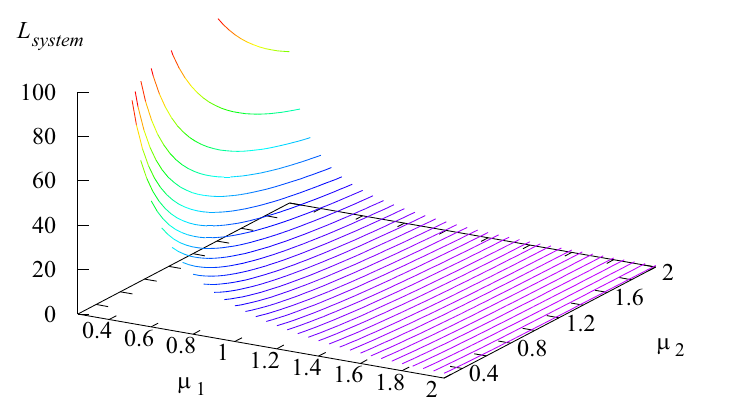
\includegraphics[width=0.8\textwidth]{CBOSr9C.png}
        \caption{Dipendenza del numero medio di clienti nel sistema $L_{\mathrm{system}}$ rispetto a $\mu_1$ e $\mu_2$ (zoomed-in)}
    \end{figure}
\end{frame}


% \begin{frame}
%     \frametitle{Terzo esempio illustrativo}
%     \begin{itemize}
%         \item La condizione di ergodicità limita il valore di $\mu_2$ per valori piccoli di $\mu_1$.
%         \item Gran parte della superficie mostrata nella prima figura è piatta a causa della violazione della condizione di ergodicità.
%         \item La tendenza generale è che $L_{\text{system}}$ diminuisce quando aumenta $\mu_1$ o $\mu_2$ (per valori non piccoli di $\mu_1$).
%     \end{itemize}
% \end{frame}


\begin{frame}
    \frametitle{Terzo esempio illustrativo}
    \begin{figure}[h]
        \centering
        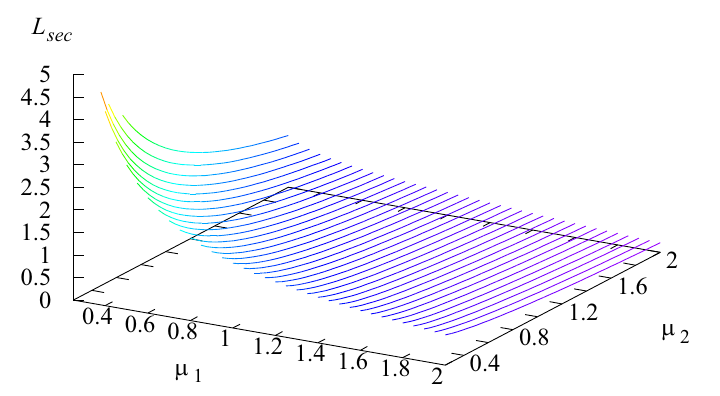
\includegraphics[width=0.8\textwidth]{R1VGHAR.png}
        \caption{Dipendenza del numero medio di clienti con server secondario $L_{\mathrm{sec}}$ rispetto a $\mu_1$ e $\mu_2$}
    \end{figure}
\end{frame}


% \begin{frame}
%     \frametitle{Terzo esempio illustrativo}
%     \begin{itemize}
%         \item Il valore massimo di $L_{sec}$ è di circa 5 quando $\mu_1$ e $\mu_2$ sono piccoli.
%         \item Con un aumento di $\mu_1$ e $\mu_2$, il valore di $L_{sec}$ diminuisce come ci si aspetterebbe.
%         \item Per valori piccoli di $\mu_1$, la diminuzione è significativa all'aumentare di $\mu_2$; per valori più grandi di $\mu_1$, notiamo un tasso insignificante di diminuzione in $L_{sec}$ con un aumento di $\mu_2$.
%     \end{itemize}
% \end{frame}


\section{Conclusioni}

% \begin{frame}
%     \frametitle{Conclusioni}
%     \begin{itemize}
%         \item Il sistema di coda analizzato prevede la possibilità di reclutare un cliente già servito come server secondario per aiutare il server principale.
%         \item Il processo di arrivo dei clienti è stato modellizzato utilizzando un processo di punto Markoviano versatile, \emph{MAP}.
%         \item È stata considerata la possibilità che i clienti insoddisfatti con il servizio fornito dal server secondario possano ritornare nel sistema.
%         \item L'analisi dello stato stazionario della catena di Markov multidimensionale ha permesso di ottenere risultati numerici utili per prendere decisioni manageriali.
%     \end{itemize}
% \end{frame}


\begin{frame}
    \frametitle{Generalizzazione del modello}
    \begin{itemize}
        \item Si può rilassare l'ipotesi di avere solo un server secondario e vedere l'impatto dell'aumento a 2.
        \item Introdurre l'ipotesi di impazienza dei clienti
        \item Incorporare la possibilità di reclutare molti server secondari con due tipi di clienti, in modo che solo un tipo possa qualificarsi per agire come server secondario.
    \end{itemize}
\end{frame}





\end{document}
